\documentclass[pdf]{beamer}
\usepackage{enumitem}
\usepackage{bm}
\setbeamertemplate{footline}[frame number]

\title{Efficient Simulation Of A Simple Evolutionary System}
\author{Mahendra Duwal Shrestha}
\institute{The University Of Tenessee}
\date{\today}


\begin{document}

  \begin{frame}
    \titlepage
  \end{frame}

  \begin{frame}
    \frametitle{Outline}
    \begin{itemize}%[\label{}]
      \item{Background}
      \item{Question 1: Distance between finite and infinite population}
      \item{Question 2: Oscillation in finite population}
      \item{Question 3: Oscillation in finite population under violation in mutation}
      \item{Question 4: Oscillation in finite population under violation in crossover}
      \item{Conclusion}
    \end{itemize}
  \end{frame}

  \begin{frame}
    \frametitle{Terms}
    \begin{itemize}
      \item{Population $P$: a collection of length $\ell$ binary strings}
      \item{Population vector $\bm{p}$: $\bm{p}_j$ is the proportion of string $j$ in the population}
      \item{If $P \,=\, {00, 01, 01, 10, 11, 11}$, then $\bm{p}_3 \,=\, 2/6 \,=\, 1/3$}
      \item{$\mathcal{R}$ denotes a set binary strings of length $\ell$ }
      \begin{itemize}
	\item{Addition and multiplication of elements in $\mathcal{R}$ are bitwise operations modulo 2}
	\item{$x \,=\, 1101,\, y \,=\, 1010 $}
	\item{$x + y \,=\, 1101 + 1010 \,=\, 0111$}
	\item{$xy \,=\, 1101 \cdot 1010 \,=\, 1000$}
	\item{$\bar{x} \,=\, 0010$}
      \end{itemize}
    \end{itemize}
  \end{frame}
  
  \begin{frame}
    \frametitle{Crossover \& Mutation}
    \begin{itemize}
      \item{Crossover : Choose parents $u$ and $v$, exchange bits using crossover mask $m$: }
      \item{$u^\prime \,=\, um + v\bar{m} , v^\prime \,=\, u\bar{m} + vm$}      
      \item{$u = \bm{11001011}, v = 11011111, m = 11110000$}
      \item{$\{\bm{11001011}, 11011111\} \to \{\bm{1100}0000 + 00001111,\; 0000\bm{1011} + 11010000\} \to \{\bm{1100}1111, 1101\bm{1011}\}$}
      \item{Mutation: Flip bits using mutation mask:}
      \item{$x \to x + m$}
    \end{itemize}
  \end{frame}
  
  \begin{frame}
    \frametitle{Finite Population GA}
    \begin{columns}
          \column{0.30\linewidth}
             \centering
             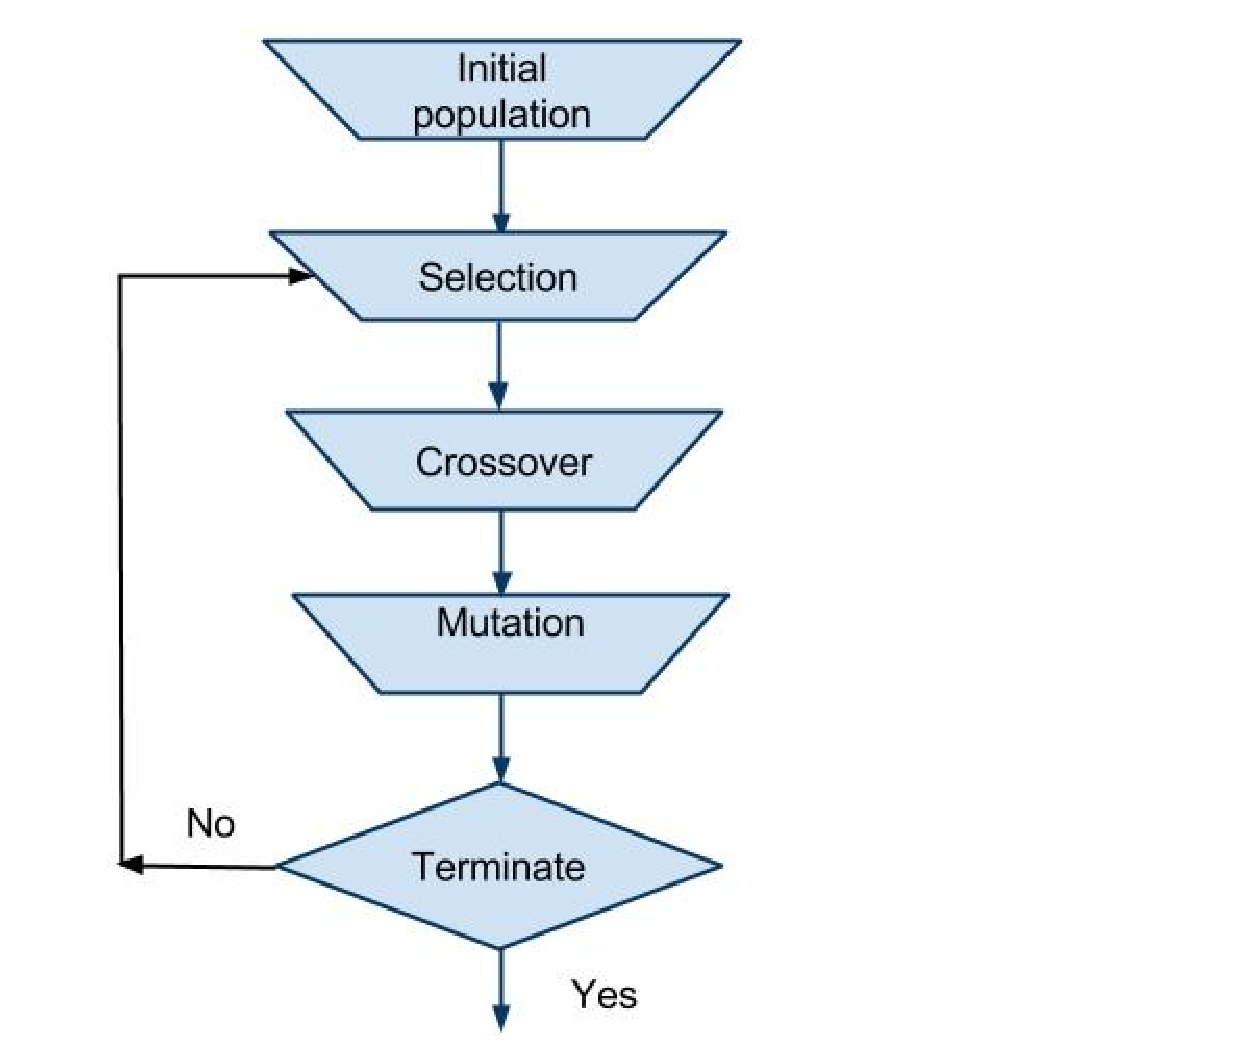
\includegraphics[height=6cm, width=7cm]{figures/eps/GA.eps}
           \column{0.66\linewidth}
	    \begin{itemize}
              \item{Randomly select parents $u$ and $v$ }
              \item{Crossover $u$ and $v$ to produce $u^\prime$ and $v^\prime$ }
              \item{Keep one of $u^\prime$, $v^\prime$ , and mutate}
              \item{Repeat above to form next generation}
              \item{Repeat whole process until system stops  to improve or threshold is reached}
	    \end{itemize}
         \end{columns} 
  \end{frame}
  
  \begin{frame}
    \frametitle{Infinite Population Model}
    \begin{itemize}
      \item{Population is modeled as a vector $\bm{p}$}
      \item{$\mathcal{G}$ maps $\bm{p}$ to the next generation}
      \item{$\mathcal{G}(\bm{p})_j$ =  probability that string $j$ occurs in the next generation}
      \item{The infinite population model is the sequence }
      \item{$\bm{p} \to \mathcal{G}(\bm{p}) \to  {\mathcal{G}}(\mathcal{G}(\bm{p})) \to \cdots $}
    \end{itemize}  
  \end{frame}
  
  \begin{frame}
    \frametitle{Random Heuristic Search}
    \begin{itemize}
      \item{$\tau$ is a stochastic transition rule that maps $\bm{p}$ to $\bm{p}$}
      \item{For a finite population, sequence $\bm{p}, \tau(\bm{p}), \tau^2(\bm{p}), \cdots $ forms Markov chain}
      \item{$\tau(\bm{p})$ cannot be predicted with certainty }
      \item{$\mathcal{G}(\bm{p})$ is the expected next generation $\mathcal{E}(\tau(\bm{p}))$}
      \item{The variance in the next generation  is}
      \item{
	$\mathcal{E}(\| \tau (\bm{p}) - \mathcal{G}(\bm{p}) \|^2) = \frac{1 - \|\mathcal{G}(\bm{p})\|^2}{r}$
      }
    \end{itemize}
  \end{frame}
  
  \begin{frame}
    \frametitle{Question 1}
    \begin{itemize}
      \item{Chebyshev's inequality $\to\, \| \tau (\bm{p}) - \mathcal{G}(\bm{p}) \| \,\leq\, \frac{k}{\sqrt{r}} $ }
      \item{Jensen's inequality  
      $\to\, \mathcal{E}(\| \tau (\bm{p}) - \mathcal{G}(\bm{p}) \| \,\leq\, \frac{\sqrt{1 - \|\mathcal{G}(\bm{p})\|^2}}{\sqrt{r}} $}
      \item{Geometric point of view $\to\, \| \tau (\bm{p}) - \mathcal{G}(\bm{p}) \| \,=\, O(r) $ }      
    \end{itemize}
    Does distance decrease in practice like $1/\sqrt{r}$?
  \end{frame}
  
  
  
  \begin{frame}
    \frametitle{History}
    \begin{itemize}
      \item{Haldane, in 1932, summarized basic population genetics  models : Wright, Fisher and Haldane}
      \item{Several people working with evolution-inspired algorithms in the 1950s and the 1960s –  
      Box (1957), Friedman(1959), Bledsoe (1961), Bremermann (1962), and Reed, Toombs and Baricelli (1967) }
      \item{In 1960s and 1970s, Holland and colleagues formalized  and promoted population based algorithms with crossover and mutation }
      \item{Vose (1999) presented efficient methods for computing with a haploid model using mask-based operators introduced by Geiringer (1944)}
    \end{itemize}
  \end{frame}
  
\end{document}